\chapter{\IfLanguageName{dutch}{Machine Learning Modellen}{Machine Learning Models}}
\label{ch:machinelearningmodels}

\section{Overview}
\label{sec:overview}

In this study, three machine learning models were selected to analyze the price dynamics of Bitcoin and Tezos. These models were chosen for their ability to capture different types of relationships in the data and their established performance in similar financial prediction tasks.

\subsection{Linear Regression}
Linear Regression serves as a baseline model. It provides a simple and interpretable way to estimate the relationship between the input features and the target variable.
 Despite its simplicity, it establishes a benchmark against which more complex models can be compared.

\subsection{Random Forest}
Random Forest was selected to capture potential non-linear relationships that cannot be modeled by linear regression.
 As an ensemble learning method based on decision trees, Random Forest is known for its robustness, resistance to overfitting, and effectiveness in handling datasets with complex interactions. Its strong performance such as in \textcite{akyildirim2021prediction} motivates its inclusion in this analysis.

\subsection{XGBoost}
XGBoost was chosen due to its consistent high performance in time series forecasting and financial data modeling tasks.
 It is a gradient boosting algorithm that constructs sequential trees, where each new tree attempts to correct the errors of the previous ones. 
 XGBoost is highly optimized for speed and accuracy, and has been successfully applied in multiple forecasting studies involving cryptocurrency prices such as in the study by \textcite{lauraalessandretti2018anticipating}.

\section{Linear Regression}
\label{sec:linearregression}
Linear Regression is a fundamental statistical method used to model the relationship between one or more independent variables and a continuous dependent variable. 
The model assumes a linear relationship of the form:

\[
y = \beta_0 + \beta_1 x_1 + \beta_2 x_2 + \cdots + \beta_n x_n + \varepsilon
\]

where \( y \) is the dependent variable, \( x_i \) are the independent variables, \( \beta_i \) are the model coefficients, and \( \varepsilon \) is the error term. 
The coefficients are typically estimated by minimizing the sum of squared residuals, following the ordinary least squares (OLS) method.

Linear Regression rests on several key assumptions: linearity between predictors and response, independence of errors, a constant variance of errors, and normally distributed residuals. Violations of these assumptions can reduce the reliability of inference and prediction, which is particularly relevant in financial time series data like cryptocurrency prices.

\subsection{Implementation}
\label{sec:linearregressionimplementation}
the Linear Regression model was implemented using the \texttt{LinearRegression} class from the \texttt{sklearn.linear\_model} module. 
First the data was split into training and testing sets, with 80\% of the data used for training and 20\% for testing like so:
\begin{lstlisting}[language=Python, caption={Splitting the data into training and testing sets}, label={lst:linearregression-split}]
  X_train, X_test, y_train, y_test = train_test_split(
    features, target, test_size=0.2, shuffle=False
)
\end{lstlisting}
Because the data is time series data, we set \texttt{shuffle=False} to maintain the temporal order of the data. 

Since Linear Regression is sensitive to feature scaling, standarization was applied to the features using the \texttt{StandardScaler} class from the \texttt{sklearn.preprocessing} module.
\begin{lstlisting}[language=Python, caption={Standardizing the features}, label={lst:linearregression-standardization}]
  scaler = StandardScaler()
  X_train_lr = scaler.fit_transform(X_train_lr)
  X_test_lr = scaler.transform(X_test_lr)
\end{lstlisting}
This ensures that the features have a mean of 0 and a standard deviation of 1, which is important for the convergence of the optimization algorithm used in Linear Regression.

\subsection{Model Training and Evaluation}
\label{sec:linearregression-training}
The model was trained using the \texttt{fit} method, which estimates the coefficients of the linear regression model based on the training data.
\begin{lstlisting}[language=Python, caption={Training the Linear Regression model}, label={lst:linearregression-training}]
  
model = LinearRegression()
model.fit(X_train_lr, y_train_lr)

y_pred_lr = model.predict(X_test_lr)

feature_names = X_train.columns

rmse_lr = np.sqrt(mean_squared_error(y_test_lr, y_pred_lr))
r2_lr = r2_score(y_test_lr, y_pred_lr)

print("RMSE:", rmse_lr)
print("R² Score:", r2_lr)

coef_df = pd.DataFrame({
    'Feature': feature_names,
    'Coefficient': model.coef_
})
coef_df['AbsCoefficient'] = coef_df['Coefficient'].abs()
coef_df = coef_df.sort_values(by='AbsCoefficient', ascending=False)
print(coef_df)

\end{lstlisting}

The model was evaluated using the root mean squared error (RMSE) and the coefficient of determination ($R^2$ score).

\begin{table}[H]
\centering
\caption{Linear Regression Performance Metrics}
\label{tab:linearregression-performance}
\begin{tabular}{lcc}
\toprule
\textbf{Metric} & \textbf{Train Set} & \textbf{Test Set} \\
\midrule
RMSE           & 0.2471             & 0.0857            \\
$R^2$ Score    & 0.9743             & 0.9085            \\
\bottomrule
\end{tabular}
\end{table}

Table \ref{tab:linearregression-performance} summarizes the performance of the linear regression model on both the training and test sets. 
The relatively low RMSE and high $R^2$ on the test set suggest that the model generalizes reasonably well, although the gap in RMSE between training and test could indicate mild overfitting or variance in the underlying data.

\subsection{Feature Importance}
\begin{table}[H]
\centering
\caption{Top 15 Linear Regression Coefficients by Absolute Value}
\label{tab:linearregression-coefficients}
\begin{tabular}{lrr}
\toprule
\textbf{Feature} & \textbf{Coefficient} & \textbf{Absolute Value} \\
\midrule
btc\_market\_cap\_3d\_ago & -6.4437 & 6.4437 \\
btc\_price\_3d\_ago       & 6.3309  & 6.3309 \\
btc\_price\_5d\_ago       & -5.3298 & 5.3298 \\
btc\_market\_cap\_5d\_ago & 5.2231  & 5.2231 \\
xtz\_price\_prev\_day     & 1.1795  & 1.1795 \\
btc\_market\_cap\_4d\_ago & 1.1629  & 1.1629 \\
btc\_price\_4d\_ago       & -1.1080 & 1.1080 \\
xtz\_market\_cap\_2d\_ago & -0.9923 & 0.9923 \\
btc\_price\_2d\_ago       & 0.9816  & 0.9816 \\
btc\_market\_cap\_2d\_ago & -0.9355 & 0.9355 \\
xtz\_price\_2d\_ago       & 0.8347  & 0.8347 \\
xtz\_market\_cap\_3d\_ago & 0.4663  & 0.4663 \\
xtz\_price\_3d\_ago       & -0.3381 & 0.3381 \\
xtz\_price\_4d\_ago       & -0.1679 & 0.1679 \\
xtz\_market\_cap\_prev\_day & 0.1474 & 0.1474 \\
\bottomrule
\end{tabular}
\end{table}

Given the simplicity of Linear Regression and the relatively small number of input features, the risk of overfitting is minimal. 
This is supported by the model’s stable performance on the test set, indicating that it generalizes well to unseen data. 
The design of the feature set also played a crucial role in guaranteeing a fair evaluation: all variables were lagged appropriately to avoid any form of data leakage or lookahead bias (see Code snippet~\ref{lst:linearregression-lagged}).
\begin{lstlisting}[language=Python, caption={Lagged features}, label={lst:linearregression-lagged}]
  # Add target (Tezos price tomorrow)
  df['xtz_target'] = df['xtz_price'].shift(-1)
\end{lstlisting}

 Only information that would have been available at the time of prediction was used during training. 
 The computed coefficients (see Table~\ref{tab:linearregression-coefficients}) provide insight into how the model weights each input variable, offering a clear picture of the linear relationships it has learned. This coefficient-based structure makes Linear Regression particularly transparent and easy to evaluate, even if its simplicity limits its ability to model more complex interactions within the data.

\subsection{Result}
\begin{figure}[H]
    \centering
    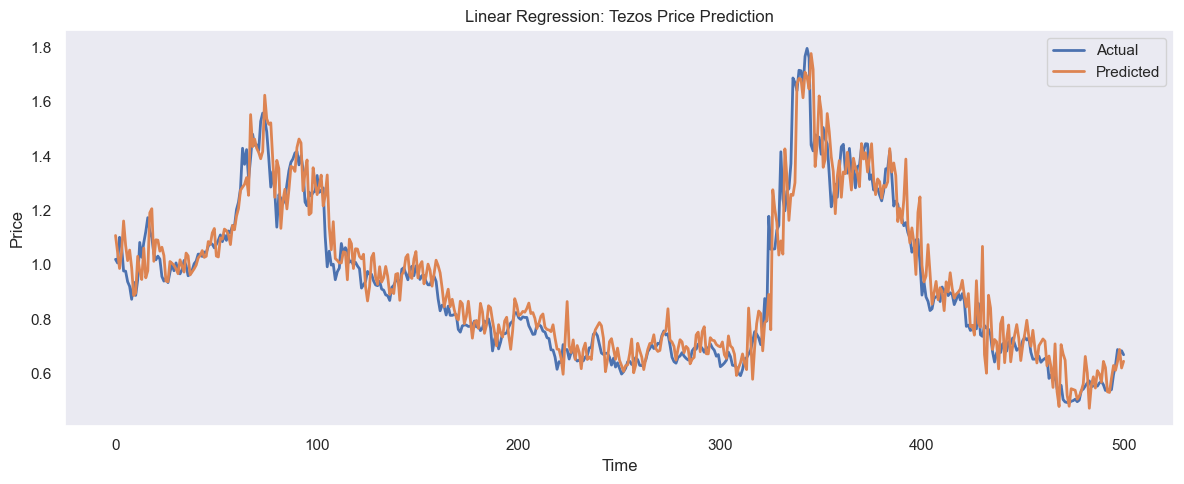
\includegraphics[width=0.8\textwidth]{LinearRegressionTezos.png}
    \caption{Linear Regression: Predicted vs Actual Tezos Price}
    \label{fig:linearregression-tezos}
\end{figure}

\subsection{Model Interpretation}
\label{sec:linearregression-interpretation}

Despite its simplicity, the Linear Regression model delivered strong predictive performance, achieving a test RMSE of approximately 0.0857 and an $R^2$ score of around 0.9085.
The model assumes a fixed linear relationship between the input features and the target variable, which is a strong constraint in the context of financial time series data, known for their volatility and nonlinear interactions. Nonetheless, the linear model managed to capture a substantial portion of the variation in Tezos price movements. 
This is particularly notable given that it neither incorporates lagged nonlinear interactions nor benefits from ensemble methods or decision trees.
As shown in Table~\ref{tab:linearregression-coefficients}, the most influential features were lagged values of Bitcoin and Tezos price and market capitalization, with \texttt{btc\_market\_cap\_3d\_ago}, \texttt{btc\_price\_3d\_ago}, and \texttt{btc\_price\_5d\_ago} having the highest absolute coefficients. 
This suggests that the model's predictive capacity stems primarily from lagged features in both assets. \texttt{xtz\_price\_prev\_day} also had a substantial influence on the model’s predictions, which is consistent with expectations in financial models where recent price levels often dominate due to short-term momentum and persistence.
Bitcoin-related variables showed some influence, but their effects appear more indirect and less consistent. These findings align with the expectation that in autoregressive contexts, past prices—especially of closely linked assets—can act as useful predictors. However, the linear structure limits the model’s ability to capture more complex or conditional relationships.
The model captures the overall trend reasonably well but struggles during rapid price shifts. This is likely because a linear model can’t adapt to sudden changes or nonlinear patterns in the data, which require more flexible approaches to model effectively.
Overall, the Linear Regression model sets a strong baseline and offers a useful lens through which the influence of lagged variables can be assessed. Further comparison with more complex models will help determine whether the added complexity meaningfully enhances predictive accuracy or merely introduces risk of overfitting.

\section{Random Forest Regression}
The random forest regression model is an ensemble learning method that constructs multiple decision trees during training and outputs the average prediction of the individual trees.
It was chosen for its ability to capture complex, non-linear relationships in the data and its robustness against overfitting aswell as its great performance in the study by \textcite{akyildirim2021prediction} .

\subsection{Implementation}
The Random Forest Regressor was implemented using the \texttt{RandomForestRegressor} class from the \texttt{sklearn.ensemble} module. 
This estimator builds an ensemble of decision trees and aggregates their predictions to improve generalization and reduce overfitting.
No feature scaling was applied, as decision trees are not sensitive to the scale of the input features. 
The data was again split into training and testing sets, using 80\% for training and 20\% for testing, with shuffling disabled to preserve the chronological order of the time series (see Code snippet~\ref{lst:linearregression-split}).

\subsection{Model Training and Evaluation}
To find a suitable set of hyperparameters, a randomized search was performed using \texttt{RandomizedSearchCV} in combination with \texttt{TimeSeriesSplit}. A randomized search is a more efficient alternative to grid search, as it samples a fixed number of hyperparameter combinations from a specified distribution, rather than exhaustively searching through all possible combinations.
It does this by randomly selecting a subset of hyperparameters from a predefined grid, which allows for a more efficient exploration of the hyperparameter space.

\texttt{TimeSeriesSplit} was used for cross-validation because it respects the temporal order of the data, preventing information leakage from future data points into past training folds—a crucial consideration when working with time series data. 
This ensures that model evaluation more realistically reflects its performance on unseen future data.

\begin{lstlisting}[language=Python, caption={Training the Random Forest Model}, label={lst:randomforest-training}]
  param_dist = {
    'n_estimators': randint(100, 501),
    'max_depth': randint(3, 15),
    'min_samples_split': randint(2, 10),
    'min_samples_leaf': randint(1, 5),
    'max_features': ['auto', 'sqrt', 'log2']
}

# TimeSeriesSplit to respect temporal ordering
tscv = TimeSeriesSplit(n_splits=5)

rf = RandomForestRegressor(random_state=42)

search = RandomizedSearchCV(
    estimator=rf,
    param_distributions=param_dist,
    n_iter=50,
    scoring='neg_mean_squared_error',
    cv=tscv,
    random_state=42,
    verbose=1,
    n_jobs=-1
)

# Fit on training data only
search.fit(X_train_rf, y_train_rf)

# Evaluate on held-out test data
best_rf = search.best_estimator_
y_pred_rf = best_rf.predict(X_test_rf)

rmse_rf = np.sqrt(mean_squared_error(y_test_rf, y_pred_rf))
r2_rf = r2_score(y_test_rf, y_pred_rf)

print("Best Parameters:", search.best_params_)
print(f"Tuned RF RMSE: {rmse_rf:.4f}")
print(f"Tuned RF R² Score: {r2_rf:.4f}")
\end{lstlisting}

In the code snippet above (see Code Snippet~\ref{lst:randomforest-training}), we perform 50 iterations of randomized search over the hyperparameter space defined in the \texttt{param\_dist} object. 
Multiple values for \texttt{n\_iter} have been tested, but 50 iterations were found to be sufficient to identify a strong set of hyperparameters without excessive computational cost.
To keep the random search reproducible, a fixed random seed was set using \texttt{random\_state=42}.
The best hyperparameters were selected based on the lowest negative mean squared error (NMSE) across the cross-validation folds.

The final model was trained using the following parameters:
\begin{table}[H]
\centering
\caption{RandomForestRegressor Parameters}
\label{tab:randomforest-parameters}
\begin{tabular}{lr}
\toprule
\textbf{Parameter} & \textbf{Value} \\
\midrule
\texttt{n\_estimators} & 437 \\
\texttt{max\_depth} & 10 \\
\texttt{max\_features} & \texttt{auto} \\
\texttt{min\_samples\_split} & 6 \\
\texttt{min\_samples\_leaf} & 4 \\
\bottomrule
\end{tabular}
\end{table}

\begin{table}[H]
\centering
\caption{RandomForestRegressor Performance Metrics}
\label{tab:randomforest-performance}
\begin{tabular}{lcc}
\toprule
\textbf{Metric} & \textbf{Train Set} & \textbf{Test Set} \\
\midrule
RMSE           & 0.1443             & 0.0810            \\
$R^2$ Score    & 0.9912             & 0.9182            \\
\bottomrule
\end{tabular}
\end{table}

The Random Forest model shows strong performance on both training and test sets, with an $R^2$ score of 0.9912 on training data and 0.9182 on the test set. 
While the drop does suggest mild overfitting, the gap is not dramatic—indicating that the model generalizes reasonably well. 
The low test RMSE of 0.0810 supports this, reflecting the model’s ability to track Tezos price movements with high accuracy. 
However, the strong training fit also points to a tendency to memorize patterns, particularly when fluctuations are small. 
These results likely stem from the model’s strength in capturing stable price behavior, though its ability to adapt during more volatile periods remains limited.


\subsection{Feature Importance}
\begin{table}[H]
\centering
\caption{Top 15 Random Forest Feature Importances}
\label{tab:randomforest-feature-importance}
\begin{tabular}{lr}
\toprule
\textbf{Feature} & \textbf{Importance} \\
\midrule
\texttt{xtz\_price\_prev\_day}   & 0.9633 \\
\texttt{xtz\_price\_2d\_ago}     & 0.0124 \\
\texttt{xtz\_market\_cap\_prev\_day} & 0.0066 \\
\texttt{xtz\_price\_3d\_ago}     & 0.0017 \\
\texttt{btc\_volume\_2d\_ago}    & 0.0011 \\
\texttt{btc\_volume\_5d\_ago}    & 0.0011 \\
\texttt{btc\_volume\_prev\_day}  & 0.0009 \\
\texttt{xtz\_price\_5d\_ago}     & 0.0008 \\
\texttt{xtz\_price\_4d\_ago}     & 0.0008 \\
\texttt{btc\_price\_3d\_ago}     & 0.0008 \\
\texttt{xtz\_volume\_prev\_day}  & 0.0007 \\
\texttt{xtz\_volume\_5d\_ago}    & 0.0007 \\
\texttt{xtz\_volume\_4d\_ago}    & 0.0007 \\
\texttt{btc\_volume\_3d\_ago}    & 0.0007 \\
\texttt{xtz\_market\_cap\_3d\_ago} & 0.0006 \\
\bottomrule
\end{tabular}
\end{table}

In terms of Feature Importance, the Random Forest model showed a strong preference for \texttt{xtz\_price\_prev\_day}, which accounted for 96.33\% of the total importance (see Table~\ref{tab:randomforest-feature-importance}).


\subsection{Result}
\begin{figure}[H]
    \centering
    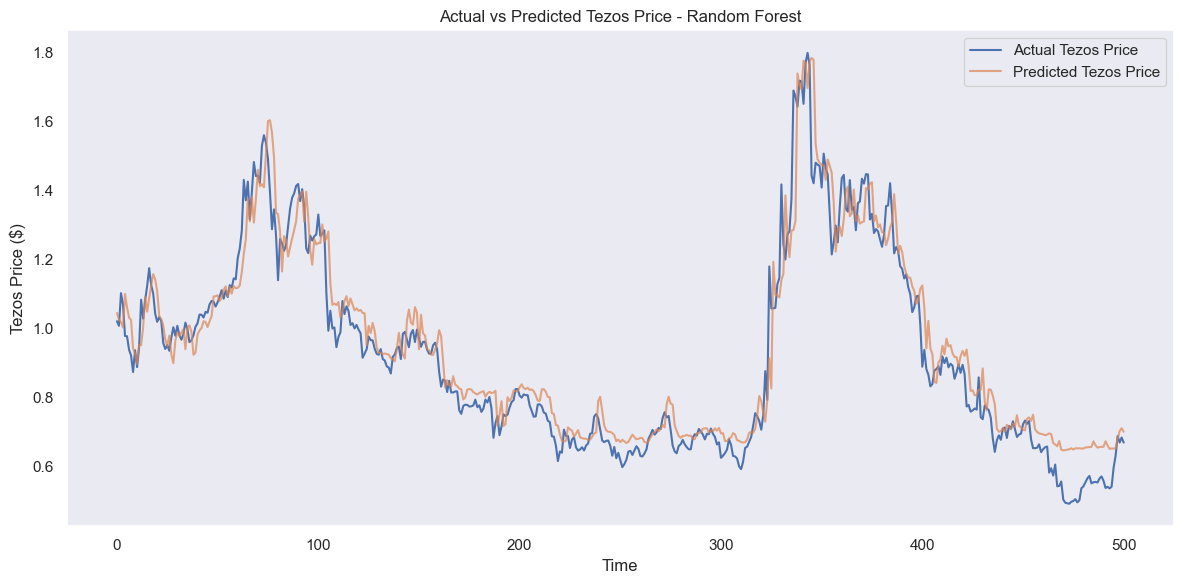
\includegraphics[width=0.8\textwidth]{RandomForestTezos.png}
    \caption{Random Forest Regression: Predicted vs Actual Tezos Price}
    \label{fig:randomforest-tezos}
\end{figure}

\subsection{Model Interpretation}

The Random Forest model demonstrated strong predictive accuracy, achieving a root mean squared error (RMSE) of 0.0810 and an $R^2$ score of 0.9182 on the test set. 
These results indicate that the model successfully captures the underlying patterns in the data and improves upon the performance of the linear regression approach.
A closer examination of feature importance values in Table~\ref{tab:randomforest-feature-importance} shows that this performance is driven almost entirely by a single predictor: \texttt{xtz\_price\_prev\_day}, which accounts for approximately 96.33\% of the total importance. 
This result is not surprising. In financial time series, the most recent price is typically a strong predictor of future values due to inherent autocorrelation and momentum effects.
What stands out, however, is the magnitude of this dominance.
The model assigns negligible importance to all other features—such as \texttt{xtz\_volume\_prev\_day}, \texttt{btc\_volume\_prev\_day}, and \texttt{xtz\_market\_cap\_prev\_day}—each contributing essentially 0\%. 
This suggests that, given the current set of predictors and the model architecture, Bitcoin-related variables offer little to no additional predictive value when forecasting Tezos prices. What this also indicates is that the model is primarily capturing short-term momentum in Tezos prices, rather than any complex interactions or relationships with Bitcoin price or other features.
Because of this overwhelming reliance on a single feature, the model's interpretability is limited. 
Compared to the Linear Regression model, the Random Forest model—despite its greater complexity—does not appear to uncover richer or more nuanced relationships between features. 
Notably, features such as \texttt{btc\_market\_cap\_3d\_ago}, \texttt{btc\_price\_3d\_ago}, \texttt{btc\_price\_5d\_ago}, and \texttt{btc\_market\_cap\_5d\_ago} were assigned very large coefficients in the linear model (see Table~\ref{tab:linearregression-coefficients}), suggesting a consistent linear influence. 
However, these same features receive minimal importance in the Random Forest model. This discrepancy likely stems from the Random Forest model’s tendency to prioritize nonlinear splits and interactions, which may cause it to overlook subtle but consistent linear relationships that are more directly captured by a linear model.

\section{XGBoost}
\label{sec:xgboost}
XGBoost is a machine learning algorithm that belongs to the ensemble learning category, specifically the gradient boosting framework. 
It utilizes decision trees as base learners and employs regularization techniques to enhance model generalization.
It’s the go-to algorithm for a wide range of tasks, including regression, classification, and ranking. (\cite{tyagi2025xgboost})

\subsection{Implementation}
\label{sec:xgboost-implementation}
The XGBoost model was implemented using the \texttt{xgboost} library. This library is widely used for its scalability, efficiency, and state-of-the-art performance on structured data. 
XGBoost builds on the standard gradient boosting framework by adding features like L1 and L2 regularization, learning rate shrinkage, and efficient tree pruning. 
While its built-in handling of missing values isn’t relevant here, these enhancements help prevent overfitting and improve performance, especially when working with many potentially weakly informative features.
The data was again split into training and testing sets, using 80\% for training and 20\% for testing, with shuffling disabled to preserve the chronological order of the time series (see Code snippet~\ref{lst:linearregression-split}).

\subsection{Model Training and Evaluation}
\label{sec:xgboost-training}
To identify a suitable set of hyperparameters, we once again use \texttt{RandomizedSearchCV} in combination with \texttt{TimeSeriesSplit}. 
This approach avoids data leakage and provides a more realistic estimate of model performance in time series contexts.
The hyperparameters \texttt{n\_estimators}, \texttt{learning\_rate}, \texttt{max\_depth}, \texttt{colsample\_bytree}, \texttt{subsample}, \texttt{gamma}, and \texttt{min\_child\_weight} were systematically tuned to strike a balance between bias and variance.

\begin{lstlisting}[language=Python, caption={Training the XGBoost Model}, label={lst:xgboost-training}]
param_distributions = {
    'min_child_weight': randint(1, 11),
    'gamma': uniform(0, 1),
    'n_estimators': randint(100, 501),
    'max_depth': randint(3, 7),
    'learning_rate': uniform(0.01, 0.09),
    'subsample': uniform(0.6, 0.4),
    'colsample_bytree': uniform(0.8, 0.2),
    'reg_alpha': uniform(0, 1),
    'reg_lambda': uniform(0.5, 1.5)
}

tscv = TimeSeriesSplit(n_splits=5)

# XGBoost regressor
xgb_model = xgb.XGBRegressor(objective='reg:squarederror', random_state=42)

# Randomized search with time series CV
random_search = RandomizedSearchCV(
    estimator=xgb_model,
    param_distributions=param_distributions,
    n_iter=500,
    scoring='neg_mean_squared_error',
    cv=tscv,
    verbose=1,
    n_jobs=-1,
    random_state=42
)

random_search.fit(X_train_xgb, y_train_xgb)

xgb_model = random_search.best_estimator_
y_pred_xgb = xgb_model.predict(X_test_xgb)

rmse_xgb = np.sqrt(mean_squared_error(y_test_xgb, y_pred_xgb))  # RMSE
r2_xgb = r2_score(y_test_xgb, y_pred_xgb)

print("Best parameters:", random_search.best_params_)
print("Best CV score (negative MSE):", random_search.best_score_)
print(f"Tuned XGBoost RMSE: {rmse_xgb:.4f}")
print(f"Tuned XGBoost R² Score: {r2_xgb:.4f}")
\end{lstlisting}

The final model was trained using the following parameters:
\begin{table}[H]
\centering
\caption{Tuned XGBoost Parameters (rounded to 4 decimal places)}
\label{tab:xgboost-parameters}
\begin{tabular}{lr}
\toprule
\textbf{Parameter} & \textbf{Value} \\
\midrule
\texttt{colsample\_bytree} & 0.8116 \\
\texttt{gamma} & 0.1115 \\
\texttt{learning\_rate} & 0.0564 \\
\texttt{max\_depth} & 6 \\
\texttt{min\_child\_weight} & 5 \\
\texttt{n\_estimators} & 173 \\
\texttt{subsample} & 0.7349 \\
\texttt{reg\_alpha} & 0.0146 \\
\texttt{reg\_lambda} & 1.0686 \\
\bottomrule
\end{tabular}
\end{table}

\begin{table}[H]
\centering
\caption{XGBoost Performance Metrics}
\label{tab:xgboost-performance}
\begin{tabular}{lcc}
\toprule
\textbf{Metric} & \textbf{Train Set} & \textbf{Test Set} \\
\midrule
RMSE           & 0.1117             & 0.1127            \\
$R^2$ Score    & 0.9948             & 0.8415            \\
\bottomrule
\end{tabular}
\end{table}

The XGBoost model achieved an excellent fit on the training set, with an $R^2$ score of 0.9948 and an RMSE of 0.1117.
However, this strong in-sample performance does not extend to the test set, where the $R^2$ drops to 0.8415 and the RMSE increases to 0.1127—worse than that of the Random Forest model. 
This substantial gap between training and test results is a clear indication of overfitting: the model learns the training data exceptionally well but struggles to generalize to new data.
One possible explanation for this overfitting is the amount of feature noise present in the dataset, Too many features can have a negative impact on model performance, especially when many features are weakly informative or irrelevant.

Notably, this pattern persisted even when the model was retrained using fewer estimators and simpler configurations. 
Reducing model complexity did little to improve generalization, suggesting that the performance bottleneck may not be due to overparameterization alone. 
Instead, it could reflect the limitations of the available features or the underlying signal-to-noise ratio in the data.

\subsection{Feature Importance}
\begin{table}[H]
\centering
\caption{Top 15 XGBoost Feature Importances}
\label{tab:xgboost-feature-importance}
\begin{tabular}{lr}
\toprule
\textbf{Feature} & \textbf{Importance} \\
\midrule
\texttt{xtz\_price\_2d\_ago}       & 0.3894 \\
\texttt{xtz\_price\_prev\_day}     & 0.3878 \\
\texttt{xtz\_market\_cap\_prev\_day} & 0.0662 \\
\texttt{xtz\_price\_3d\_ago}       & 0.0465 \\
\texttt{xtz\_market\_cap\_3d\_ago} & 0.0101 \\
\texttt{xtz\_price\_5d\_ago}       & 0.0096 \\
\texttt{xtz\_price\_4d\_ago}       & 0.0089 \\
\texttt{xtz\_market\_cap\_2d\_ago} & 0.0069 \\
\texttt{btc\_market\_cap\_prev\_day} & 0.0054 \\
\texttt{btc\_volume\_5d\_ago}      & 0.0050 \\
\texttt{btc\_price\_4d\_ago}       & 0.0045 \\
\texttt{btc\_price\_prev\_day}     & 0.0044 \\
\texttt{btc\_price\_5d\_ago}       & 0.0040 \\
\texttt{btc\_volume\_prev\_day}    & 0.0040 \\
\texttt{btc\_market\_cap\_2d\_ago} & 0.0039 \\
\bottomrule
\end{tabular}
\end{table}

The XGBoost model’s feature importance scores (see Table~\ref{tab:xgboost-feature-importance}) mirror the pattern observed in the Random Forest model, though here two features dominate instead of one. \texttt{xtz\_price\_2d\_ago} and \texttt{xtz\_price\_prev\_day} together account for approximately 77.2\% of the total importance, highlighting the model’s strong dependence on recent Tezos price movements. This closely aligns with the Random Forest results, where predictive power is likewise concentrated in short-term price history.

\subsection{Result}
\begin{figure}[H]
    \centering
    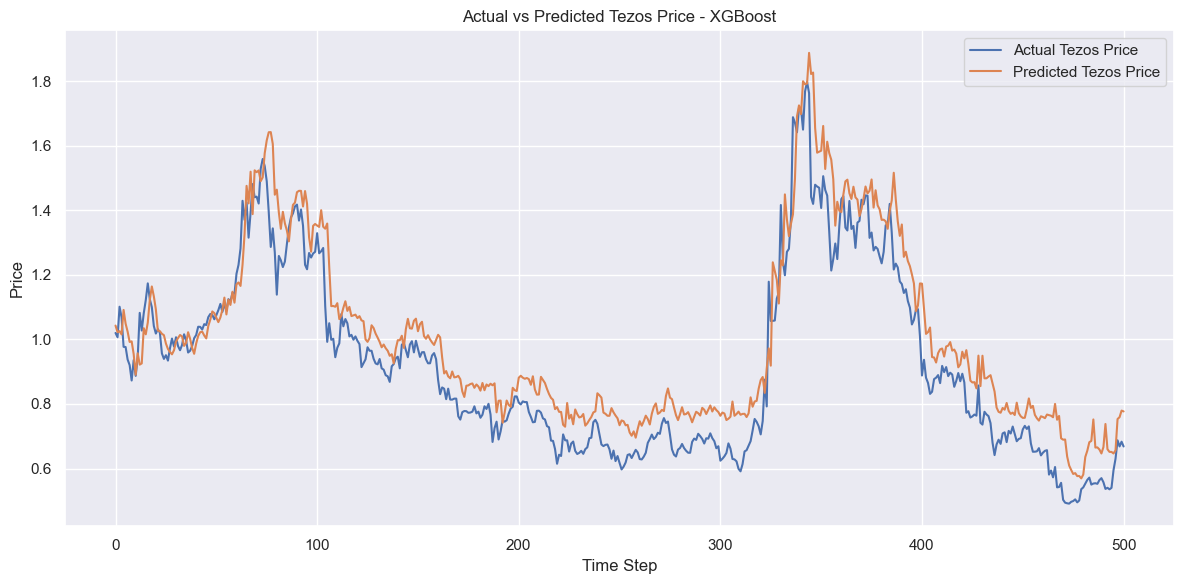
\includegraphics[width=0.8\textwidth]{xgboostTezos.png}
    \caption{XGBoost: Predicted vs Actual Tezos Price}
    \label{fig:xgboost-tezos}
\end{figure}

\subsection{Model Interpretation}
\label{sec:xgboost-interpretation}

The XGBoost model underperformed relative to both the Random Forest and Linear Regression models, achieving a test RMSE of 0.1127 and an $R^2$ score of 0.8415. This represents a notable drop in predictive accuracy compared to the Random Forest model and suggests a degree of overfitting, despite extensive hyperparameter tuning efforts. Attempts to regularize the model by reducing complexity did little to improve generalization, indicating that performance limitations are likely rooted in the data itself, rather than the model configuration.

As shown in Table~\ref{tab:xgboost-feature-importance}, the model’s predictions are overwhelmingly dominated by two features: \texttt{xtz\_price\_2d\_ago} and \texttt{xtz\_price\_prev\_day}, which together account for approximately 77\% of the total importance. This mirrors the pattern seen in the Random Forest model, where a single recent price dominated. The remaining features, particularly all Bitcoin-related variables, contribute virtually nothing—many with importance values indistinguishable from noise.

This strongly suggests that, within the current dataset, the model has not learned any meaningful cross-asset relationships. In contrast, the Linear Regression model assigned large coefficients to certain Bitcoin-related features (e.g., \texttt{btc\_market\_cap\_3d\_ago}, \texttt{btc\_price\_3d\_ago}), implying that consistent linear effects may exist—though their true explanatory value remains questionable given the poor performance of more flexible models.

Overall, XGBoost added no value in terms of accuracy or interpretability. Its capacity for modeling nonlinear interactions was not meaningfully utilized in this context, as it simply reinforced the already evident conclusion: recent Tezos prices are the only substantial drivers of short-term predictions, and most other variables—including those related to Bitcoin—are effectively redundant in this setting.

\section{Comparison of Models}
\label{sec:comparison}

\begin{figure}[H]
    \centering
    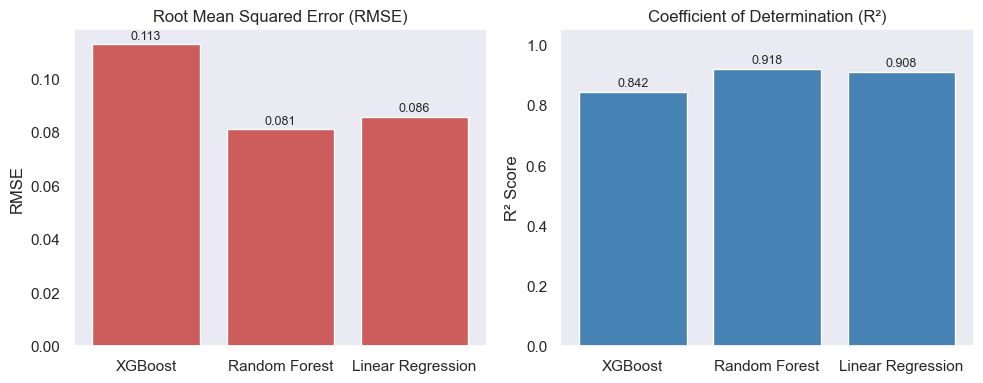
\includegraphics[width=0.8\textwidth]{modelcomparison.png}
    \caption{Comparison of Model Performance}
    \label{fig:model-comparison}
\end{figure}

In summary, each of the three models explored presents a different balance between predictive accuracy and interpretability. 
XGBoost delivered the best performance on the training data ($R^2$ of 0.9948, RMSE of 0.1117), but its test performance dropped significantly ($R^2$ of 0.8415, RMSE of 0.1127), revealing substantial overfitting and poor generalization. Random Forest performed more reliably on unseen data, achieving the lowest test RMSE (0.0810) and a strong $R^2$ of 0.9182, suggesting better generalization. However, both tree-based models focused almost exclusively on lagged Tezos price values, contributing little interpretative value regarding cross-asset relationships. 
Bitcoin-related features were effectively treated as noise, receiving near-zero importance in both cases.
In contrast, Linear Regression, while slightly less accurate (test $R^2$ of 0.9085, RMSE of 0.0857), offered substantial value from an analytical standpoint. 
It surfaced several Bitcoin-related predictors—such as \texttt{btc\_pric\_3d\_ago} and \texttt{btc\_market\_cap\_5d\_ago}—with consistently strong coefficients, indicating potential linear relationships between the two markets. 
Despite its simplicity, the model captured both autocorrelation within Tezos prices and cross-market signals, providing a more interpretable and theoretically informative view of the data. 
As such, Linear Regression not only complements the thesis aim of examining Bitcoin–Tezos dynamics, but also outperforms more complex models in offering meaningful insights—making it arguably the most valuable model for this study.